\begin{frame}[fragile]{Exemplo de remoção no caso 1.2, $m = 4$}

    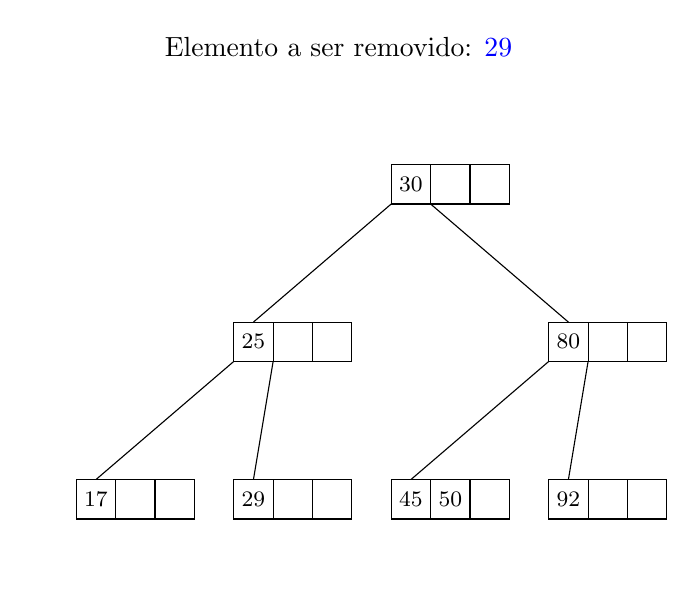
\begin{tikzpicture}
        \begin{scope}
            \node[opacity=0] at (-0.5, -0.5) { } ;
            \node[anchor=west] at (1, 6.0) { Elemento a ser removido: \textcolor{blue}{29} };

            \draw (4, 4) rectangle (4.5, 4.5);
            \draw (4.5, 4) rectangle (5, 4.5);
            \draw (5, 4) rectangle (5.5, 4.5);

            \draw (2, 2) rectangle (2.5, 2.5);
            \draw (2.5, 2) rectangle (3, 2.5);
            \draw (3, 2) rectangle (3.5, 2.5);

            \draw (6, 2) rectangle (6.5, 2.5);
            \draw (6.5, 2) rectangle (7, 2.5);
            \draw (7, 2) rectangle (7.5, 2.5);

            \draw (0, 0) rectangle (0.5, 0.5);
            \draw (0.5, 0) rectangle (1, 0.5);
            \draw (1, 0) rectangle (1.5, 0.5);

            \draw (2, 0) rectangle (2.5, 0.5);
            \draw (2.5, 0) rectangle (3, 0.5);
            \draw (3, 0) rectangle (3.5, 0.5);

            \draw (4, 0) rectangle (4.5, 0.5);
            \draw (4.5, 0) rectangle (5, 0.5);
            \draw (5, 0) rectangle (5.5, 0.5);

            \draw (6, 0) rectangle (6.5, 0.5);
            \draw (6.5, 0) rectangle (7, 0.5);
            \draw (7, 0) rectangle (7.5, 0.5);

            \node at (4.25, 4.25) { \footnotesize \textcolor{black}{30} };

            \node at (2.25, 2.25) { \footnotesize \textcolor{black}{25} };

            \node at (6.25, 2.25) { \footnotesize \textcolor{black}{80} };

            \node at (0.25, 0.25) { \footnotesize \textcolor{black}{17} };

            \node at (2.25, 0.25) { \footnotesize \textcolor{black}{29} };

            \node at (4.25, 0.25) { \footnotesize \textcolor{black}{45} };
            \node at (4.75, 0.25) { \footnotesize \textcolor{black}{50} };

            \node at (6.25, 0.25) { \footnotesize \textcolor{black}{92} };

            \draw (4,4) -- (2.25, 2.5);
            \draw (4.5,4) -- (6.25, 2.5);

            \draw (2,2) -- (0.25, 0.5);
            \draw (2.5,2) -- (2.25, 0.5);
            \draw (6,2) -- (4.25, 0.5);
            \draw (6.5,2) -- (6.25, 0.5);

        \end{scope}
 
    \end{tikzpicture}
\end{frame}

\begin{frame}[fragile]{Exemplo de remoção no caso 1.2, $m = 4$}

    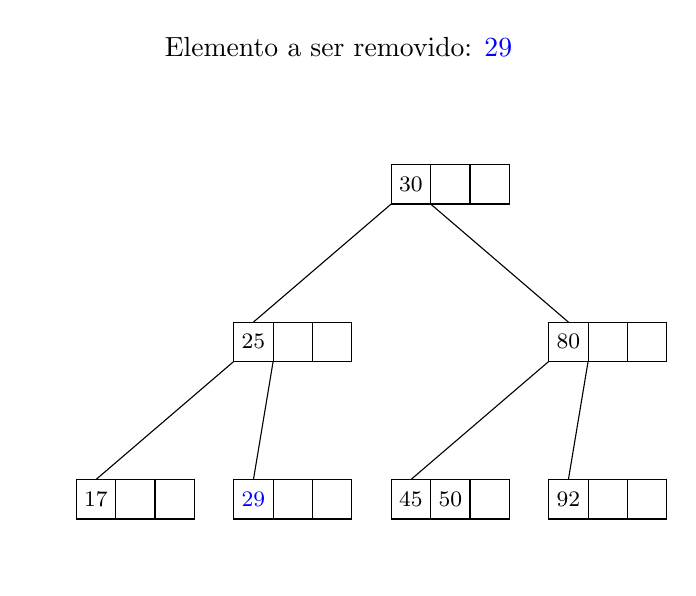
\begin{tikzpicture}
        \begin{scope}
            \node[opacity=0] at (-0.5, -0.5) { } ;
            \node[anchor=west] at (1, 6.0) { Elemento a ser removido: \textcolor{blue}{29} };

            \draw (4, 4) rectangle (4.5, 4.5);
            \draw (4.5, 4) rectangle (5, 4.5);
            \draw (5, 4) rectangle (5.5, 4.5);

            \draw (2, 2) rectangle (2.5, 2.5);
            \draw (2.5, 2) rectangle (3, 2.5);
            \draw (3, 2) rectangle (3.5, 2.5);

            \draw (6, 2) rectangle (6.5, 2.5);
            \draw (6.5, 2) rectangle (7, 2.5);
            \draw (7, 2) rectangle (7.5, 2.5);

            \draw (0, 0) rectangle (0.5, 0.5);
            \draw (0.5, 0) rectangle (1, 0.5);
            \draw (1, 0) rectangle (1.5, 0.5);

            \draw (2, 0) rectangle (2.5, 0.5);
            \draw (2.5, 0) rectangle (3, 0.5);
            \draw (3, 0) rectangle (3.5, 0.5);

            \draw (4, 0) rectangle (4.5, 0.5);
            \draw (4.5, 0) rectangle (5, 0.5);
            \draw (5, 0) rectangle (5.5, 0.5);

            \draw (6, 0) rectangle (6.5, 0.5);
            \draw (6.5, 0) rectangle (7, 0.5);
            \draw (7, 0) rectangle (7.5, 0.5);

            \node at (4.25, 4.25) { \footnotesize \textcolor{black}{30} };

            \node at (2.25, 2.25) { \footnotesize \textcolor{black}{25} };

            \node at (6.25, 2.25) { \footnotesize \textcolor{black}{80} };

            \node at (0.25, 0.25) { \footnotesize \textcolor{black}{17} };

            \node at (2.25, 0.25) { \footnotesize \textcolor{blue}{29} };

            \node at (4.25, 0.25) { \footnotesize \textcolor{black}{45} };
            \node at (4.75, 0.25) { \footnotesize \textcolor{black}{50} };

            \node at (6.25, 0.25) { \footnotesize \textcolor{black}{92} };

            \draw (4,4) -- (2.25, 2.5);
            \draw (4.5,4) -- (6.25, 2.5);

            \draw (2,2) -- (0.25, 0.5);
            \draw (2.5,2) -- (2.25, 0.5);
            \draw (6,2) -- (4.25, 0.5);
            \draw (6.5,2) -- (6.25, 0.5);

        \end{scope}
 
    \end{tikzpicture}
\end{frame}

\begin{frame}[fragile]{Exemplo de remoção no caso 1.2, $m = 4$}

    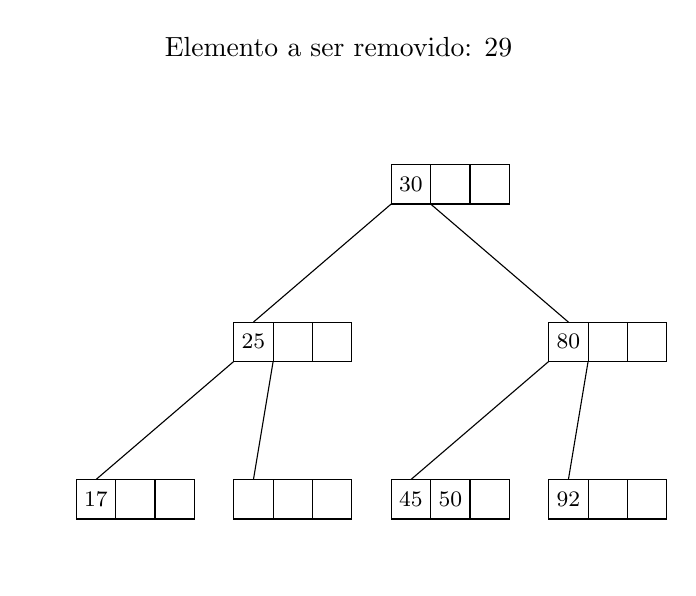
\begin{tikzpicture}
        \begin{scope}
            \node[opacity=0] at (-0.5, -0.5) { } ;
            \node[anchor=west] at (1, 6.0) { Elemento a ser removido: \textcolor{black}{29} };

            \draw (4, 4) rectangle (4.5, 4.5);
            \draw (4.5, 4) rectangle (5, 4.5);
            \draw (5, 4) rectangle (5.5, 4.5);

            \draw (2, 2) rectangle (2.5, 2.5);
            \draw (2.5, 2) rectangle (3, 2.5);
            \draw (3, 2) rectangle (3.5, 2.5);

            \draw (6, 2) rectangle (6.5, 2.5);
            \draw (6.5, 2) rectangle (7, 2.5);
            \draw (7, 2) rectangle (7.5, 2.5);

            \draw (0, 0) rectangle (0.5, 0.5);
            \draw (0.5, 0) rectangle (1, 0.5);
            \draw (1, 0) rectangle (1.5, 0.5);

            \draw (2, 0) rectangle (2.5, 0.5);
            \draw (2.5, 0) rectangle (3, 0.5);
            \draw (3, 0) rectangle (3.5, 0.5);

            \draw (4, 0) rectangle (4.5, 0.5);
            \draw (4.5, 0) rectangle (5, 0.5);
            \draw (5, 0) rectangle (5.5, 0.5);

            \draw (6, 0) rectangle (6.5, 0.5);
            \draw (6.5, 0) rectangle (7, 0.5);
            \draw (7, 0) rectangle (7.5, 0.5);

            \node at (4.25, 4.25) { \footnotesize \textcolor{black}{30} };

            \node at (2.25, 2.25) { \footnotesize \textcolor{black}{25} };

            \node at (6.25, 2.25) { \footnotesize \textcolor{black}{80} };

            \node at (0.25, 0.25) { \footnotesize \textcolor{black}{17} };

            \node at (4.25, 0.25) { \footnotesize \textcolor{black}{45} };
            \node at (4.75, 0.25) { \footnotesize \textcolor{black}{50} };

            \node at (6.25, 0.25) { \footnotesize \textcolor{black}{92} };

            \draw (4,4) -- (2.25, 2.5);
            \draw (4.5,4) -- (6.25, 2.5);

            \draw (2,2) -- (0.25, 0.5);
            \draw (2.5,2) -- (2.25, 0.5);
            \draw (6,2) -- (4.25, 0.5);
            \draw (6.5,2) -- (6.25, 0.5);

        \end{scope}
 
    \end{tikzpicture}
\end{frame}

\begin{frame}[fragile]{Exemplo de remoção no caso 1.2, $m = 4$}

    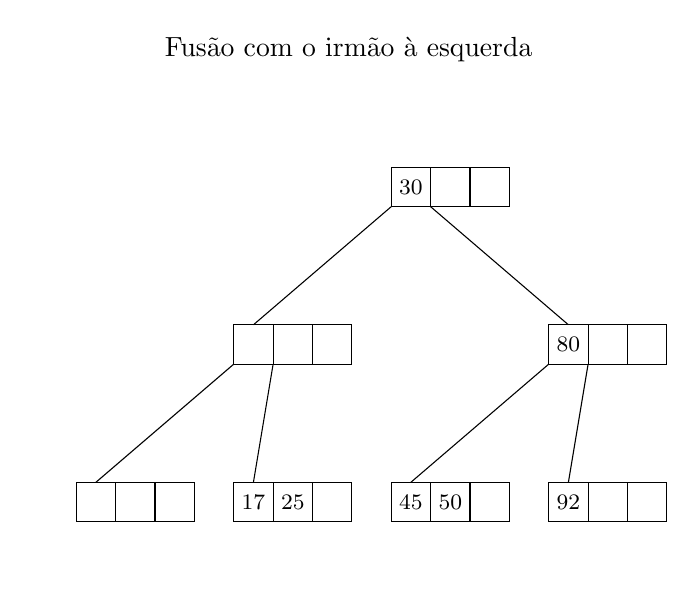
\begin{tikzpicture}
        \begin{scope}
            \node[opacity=0] at (-0.5, -0.5) { } ;
            \node[anchor=west] at (1, 6.0) { Fusão com o irmão à esquerda };

            \draw (4, 4) rectangle (4.5, 4.5);
            \draw (4.5, 4) rectangle (5, 4.5);
            \draw (5, 4) rectangle (5.5, 4.5);

            \draw (2, 2) rectangle (2.5, 2.5);
            \draw (2.5, 2) rectangle (3, 2.5);
            \draw (3, 2) rectangle (3.5, 2.5);

            \draw (6, 2) rectangle (6.5, 2.5);
            \draw (6.5, 2) rectangle (7, 2.5);
            \draw (7, 2) rectangle (7.5, 2.5);

            \draw (0, 0) rectangle (0.5, 0.5);
            \draw (0.5, 0) rectangle (1, 0.5);
            \draw (1, 0) rectangle (1.5, 0.5);

            \draw (2, 0) rectangle (2.5, 0.5);
            \draw (2.5, 0) rectangle (3, 0.5);
            \draw (3, 0) rectangle (3.5, 0.5);

            \draw (4, 0) rectangle (4.5, 0.5);
            \draw (4.5, 0) rectangle (5, 0.5);
            \draw (5, 0) rectangle (5.5, 0.5);

            \draw (6, 0) rectangle (6.5, 0.5);
            \draw (6.5, 0) rectangle (7, 0.5);
            \draw (7, 0) rectangle (7.5, 0.5);

            \node at (4.25, 4.25) { \footnotesize \textcolor{black}{30} };


            \node at (6.25, 2.25) { \footnotesize \textcolor{black}{80} };

            \node at (2.25, 0.25) { \footnotesize \textcolor{black}{17} };
            \node at (2.75, 0.25) { \footnotesize \textcolor{black}{25} };

            \node at (4.25, 0.25) { \footnotesize \textcolor{black}{45} };
            \node at (4.75, 0.25) { \footnotesize \textcolor{black}{50} };

            \node at (6.25, 0.25) { \footnotesize \textcolor{black}{92} };

            \draw (4,4) -- (2.25, 2.5);
            \draw (4.5,4) -- (6.25, 2.5);

            \draw (2,2) -- (0.25, 0.5);
            \draw (2.5,2) -- (2.25, 0.5);
            \draw (6,2) -- (4.25, 0.5);
            \draw (6.5,2) -- (6.25, 0.5);

        \end{scope}
 
    \end{tikzpicture}
\end{frame}

\begin{frame}[fragile]{Exemplo de remoção no caso 1.2, $m = 4$}

    \begin{tikzpicture}
        \begin{scope}
            \node[opacity=0] at (-0.5, -0.5) { } ;
            \node[anchor=west] at (1, 6.0) { Fusão com o irmão à esquerda };

            \draw (4, 4) rectangle (4.5, 4.5);
            \draw (4.5, 4) rectangle (5, 4.5);
            \draw (5, 4) rectangle (5.5, 4.5);

            \draw (2, 2) rectangle (2.5, 2.5);
            \draw (2.5, 2) rectangle (3, 2.5);
            \draw (3, 2) rectangle (3.5, 2.5);

            \draw (6, 2) rectangle (6.5, 2.5);
            \draw (6.5, 2) rectangle (7, 2.5);
            \draw (7, 2) rectangle (7.5, 2.5);

            \draw (2, 0) rectangle (2.5, 0.5);
            \draw (2.5, 0) rectangle (3, 0.5);
            \draw (3, 0) rectangle (3.5, 0.5);

            \draw (4, 0) rectangle (4.5, 0.5);
            \draw (4.5, 0) rectangle (5, 0.5);
            \draw (5, 0) rectangle (5.5, 0.5);

            \draw (6, 0) rectangle (6.5, 0.5);
            \draw (6.5, 0) rectangle (7, 0.5);
            \draw (7, 0) rectangle (7.5, 0.5);

            \node at (4.25, 4.25) { \footnotesize \textcolor{black}{30} };

            \node at (6.25, 2.25) { \footnotesize \textcolor{black}{80} };

            \node at (2.25, 0.25) { \footnotesize \textcolor{black}{17} };
            \node at (2.75, 0.25) { \footnotesize \textcolor{black}{25} };

            \node at (4.25, 0.25) { \footnotesize \textcolor{black}{45} };
            \node at (4.75, 0.25) { \footnotesize \textcolor{black}{50} };

            \node at (6.25, 0.25) { \footnotesize \textcolor{black}{92} };

            \draw (4,4) -- (2.25, 2.5);
            \draw (4.5,4) -- (6.25, 2.5);

            \draw (2.5,2) -- (2.25, 0.5);
            \draw (6,2) -- (4.25, 0.5);
            \draw (6.5,2) -- (6.25, 0.5);

        \end{scope}
 
    \end{tikzpicture}
\end{frame}

\begin{frame}[fragile]{Exemplo de remoção no caso 1.2, $m = 4$}

    \begin{tikzpicture}
        \begin{scope}
            \node[opacity=0] at (-0.5, -0.5) { } ;
            \node[anchor=west] at (1, 6.0) { Violação das propriedades no pai: correção no nível superior };

            \draw (4, 4) rectangle (4.5, 4.5);
            \draw (4.5, 4) rectangle (5, 4.5);
            \draw (5, 4) rectangle (5.5, 4.5);

            \draw (2, 2) rectangle (2.5, 2.5);
            \draw (2.5, 2) rectangle (3, 2.5);
            \draw (3, 2) rectangle (3.5, 2.5);

            \draw (6, 2) rectangle (6.5, 2.5);
            \draw (6.5, 2) rectangle (7, 2.5);
            \draw (7, 2) rectangle (7.5, 2.5);

            \draw (2, 0) rectangle (2.5, 0.5);
            \draw (2.5, 0) rectangle (3, 0.5);
            \draw (3, 0) rectangle (3.5, 0.5);

            \draw (4, 0) rectangle (4.5, 0.5);
            \draw (4.5, 0) rectangle (5, 0.5);
            \draw (5, 0) rectangle (5.5, 0.5);

            \draw (6, 0) rectangle (6.5, 0.5);
            \draw (6.5, 0) rectangle (7, 0.5);
            \draw (7, 0) rectangle (7.5, 0.5);

            \node at (4.25, 4.25) { \footnotesize \textcolor{black}{30} };

            \node at (6.25, 2.25) { \footnotesize \textcolor{black}{80} };

            \node at (2.25, 0.25) { \footnotesize \textcolor{black}{17} };
            \node at (2.75, 0.25) { \footnotesize \textcolor{black}{25} };

            \node at (4.25, 0.25) { \footnotesize \textcolor{black}{45} };
            \node at (4.75, 0.25) { \footnotesize \textcolor{black}{50} };

            \node at (6.25, 0.25) { \footnotesize \textcolor{black}{92} };

            \draw (4,4) -- (2.25, 2.5);
            \draw (4.5,4) -- (6.25, 2.5);

            \draw (2.5,2) -- (2.25, 0.5);
            \draw (6,2) -- (4.25, 0.5);
            \draw (6.5,2) -- (6.25, 0.5);

        \end{scope}
 
    \end{tikzpicture}
\end{frame}

\begin{frame}[fragile]{Exemplo de remoção no caso 1.2, $m = 4$}

    \begin{tikzpicture}
        \begin{scope}
            \node[opacity=0] at (-0.5, -0.5) { } ;
            \node[anchor=west] at (1, 6.0) { Fusão com o irmão à direita };

            \draw (4, 4) rectangle (4.5, 4.5);
            \draw (4.5, 4) rectangle (5, 4.5);
            \draw (5, 4) rectangle (5.5, 4.5);

            \draw (2, 2) rectangle (2.5, 2.5);
            \draw (2.5, 2) rectangle (3, 2.5);
            \draw (3, 2) rectangle (3.5, 2.5);

            \draw (6, 2) rectangle (6.5, 2.5);
            \draw (6.5, 2) rectangle (7, 2.5);
            \draw (7, 2) rectangle (7.5, 2.5);

            \draw (2, 0) rectangle (2.5, 0.5);
            \draw (2.5, 0) rectangle (3, 0.5);
            \draw (3, 0) rectangle (3.5, 0.5);

            \draw (4, 0) rectangle (4.5, 0.5);
            \draw (4.5, 0) rectangle (5, 0.5);
            \draw (5, 0) rectangle (5.5, 0.5);

            \draw (6, 0) rectangle (6.5, 0.5);
            \draw (6.5, 0) rectangle (7, 0.5);
            \draw (7, 0) rectangle (7.5, 0.5);

            \node at (2.25, 2.25) { \footnotesize \textcolor{black}{30} };
            \node at (2.75, 2.25) { \footnotesize \textcolor{black}{80} };

            \node at (2.25, 0.25) { \footnotesize \textcolor{black}{17} };
            \node at (2.75, 0.25) { \footnotesize \textcolor{black}{25} };

            \node at (4.25, 0.25) { \footnotesize \textcolor{black}{45} };
            \node at (4.75, 0.25) { \footnotesize \textcolor{black}{50} };

            \node at (6.25, 0.25) { \footnotesize \textcolor{black}{92} };

            \draw (4,4) -- (2.25, 2.5);
            \draw (4.5,4) -- (6.25, 2.5);

            \draw (2,2) -- (2.25, 0.5);
            \draw (6,2) -- (4.25, 0.5);
            \draw (6.5,2) -- (6.25, 0.5);

        \end{scope}
 
    \end{tikzpicture}
\end{frame}

\begin{frame}[fragile]{Exemplo de remoção no caso 1.2, $m = 4$}

    \begin{tikzpicture}
        \begin{scope}
            \node[opacity=0] at (-0.5, -0.5) { } ;
            \node[anchor=west] at (1, 6.0) { Fusão com o irmão à direita };

            \draw (4, 4) rectangle (4.5, 4.5);
            \draw (4.5, 4) rectangle (5, 4.5);
            \draw (5, 4) rectangle (5.5, 4.5);

            \draw (4, 2) rectangle (4.5, 2.5);
            \draw (4.5, 2) rectangle (5, 2.5);
            \draw (5, 2) rectangle (5.5, 2.5);

            \draw (2, 0) rectangle (2.5, 0.5);
            \draw (2.5, 0) rectangle (3, 0.5);
            \draw (3, 0) rectangle (3.5, 0.5);

            \draw (4, 0) rectangle (4.5, 0.5);
            \draw (4.5, 0) rectangle (5, 0.5);
            \draw (5, 0) rectangle (5.5, 0.5);

            \draw (6, 0) rectangle (6.5, 0.5);
            \draw (6.5, 0) rectangle (7, 0.5);
            \draw (7, 0) rectangle (7.5, 0.5);

            \node at (4.25, 2.25) { \footnotesize \textcolor{black}{30} };
            \node at (4.75, 2.25) { \footnotesize \textcolor{black}{80} };

            \node at (2.25, 0.25) { \footnotesize \textcolor{black}{17} };
            \node at (2.75, 0.25) { \footnotesize \textcolor{black}{25} };

            \node at (4.25, 0.25) { \footnotesize \textcolor{black}{45} };
            \node at (4.75, 0.25) { \footnotesize \textcolor{black}{50} };

            \node at (6.25, 0.25) { \footnotesize \textcolor{black}{92} };

            \draw (4,4) -- (4.25, 2.5);

            \draw (4,2) -- (2.25, 0.5);
            \draw (4.5,2) -- (4.25, 0.5);
            \draw (5,2) -- (6.25, 0.5);

        \end{scope}
 
    \end{tikzpicture}
\end{frame}

\begin{frame}[fragile]{Exemplo de remoção no caso 1.2, $m = 4$}

    \begin{tikzpicture}
        \begin{scope}
            \node[opacity=0] at (-0.5, -0.5) { } ;
            \node[anchor=west] at (1, 6.0) { Violação na raiz: correção no nível superior };

            \draw (4, 4) rectangle (4.5, 4.5);
            \draw (4.5, 4) rectangle (5, 4.5);
            \draw (5, 4) rectangle (5.5, 4.5);

            \draw (4, 2) rectangle (4.5, 2.5);
            \draw (4.5, 2) rectangle (5, 2.5);
            \draw (5, 2) rectangle (5.5, 2.5);

            \draw (2, 0) rectangle (2.5, 0.5);
            \draw (2.5, 0) rectangle (3, 0.5);
            \draw (3, 0) rectangle (3.5, 0.5);

            \draw (4, 0) rectangle (4.5, 0.5);
            \draw (4.5, 0) rectangle (5, 0.5);
            \draw (5, 0) rectangle (5.5, 0.5);

            \draw (6, 0) rectangle (6.5, 0.5);
            \draw (6.5, 0) rectangle (7, 0.5);
            \draw (7, 0) rectangle (7.5, 0.5);

            \node at (4.25, 2.25) { \footnotesize \textcolor{black}{30} };
            \node at (4.75, 2.25) { \footnotesize \textcolor{black}{80} };

            \node at (2.25, 0.25) { \footnotesize \textcolor{black}{17} };
            \node at (2.75, 0.25) { \footnotesize \textcolor{black}{25} };

            \node at (4.25, 0.25) { \footnotesize \textcolor{black}{45} };
            \node at (4.75, 0.25) { \footnotesize \textcolor{black}{50} };

            \node at (6.25, 0.25) { \footnotesize \textcolor{black}{92} };

            \draw (4,4) -- (4.25, 2.5);

            \draw (4,2) -- (2.25, 0.5);
            \draw (4.5,2) -- (4.25, 0.5);
            \draw (5,2) -- (6.25, 0.5);

        \end{scope}
 
    \end{tikzpicture}
\end{frame}

\begin{frame}[fragile]{Exemplo de remoção no caso 1.2, $m = 4$}

    \begin{tikzpicture}
        \begin{scope}
            \node[opacity=0] at (-0.5, -0.5) { } ;
            \node[anchor=west] at (1, 6.0) { Redução da altura da árvore: nova raiz };

            \draw (4, 2) rectangle (4.5, 2.5);
            \draw (4.5, 2) rectangle (5, 2.5);
            \draw (5, 2) rectangle (5.5, 2.5);

            \draw (2, 0) rectangle (2.5, 0.5);
            \draw (2.5, 0) rectangle (3, 0.5);
            \draw (3, 0) rectangle (3.5, 0.5);

            \draw (4, 0) rectangle (4.5, 0.5);
            \draw (4.5, 0) rectangle (5, 0.5);
            \draw (5, 0) rectangle (5.5, 0.5);

            \draw (6, 0) rectangle (6.5, 0.5);
            \draw (6.5, 0) rectangle (7, 0.5);
            \draw (7, 0) rectangle (7.5, 0.5);

            \node at (4.25, 2.25) { \footnotesize \textcolor{black}{30} };
            \node at (4.75, 2.25) { \footnotesize \textcolor{black}{80} };

            \node at (2.25, 0.25) { \footnotesize \textcolor{black}{17} };
            \node at (2.75, 0.25) { \footnotesize \textcolor{black}{25} };

            \node at (4.25, 0.25) { \footnotesize \textcolor{black}{45} };
            \node at (4.75, 0.25) { \footnotesize \textcolor{black}{50} };

            \node at (6.25, 0.25) { \footnotesize \textcolor{black}{92} };

            \draw (4,2) -- (2.25, 0.5);
            \draw (4.5,2) -- (4.25, 0.5);
            \draw (5,2) -- (6.25, 0.5);

        \end{scope}
 
    \end{tikzpicture}
\end{frame}
